\documentclass[{../../master}]{subfiles}
\graphicspath{{../..}}  % 個別コンパイル時の画像パスを解決する

\begin{document}

\section{Ubuntu 18.04LTSのインストール}

この節ではIntel NUCへUbuntu 18.04LTSをインストールする手順を説明します.
尚,NUCの組み立ては完了しているものとします.

\subsection{必要なもの}

Ubuntuのインストール作業には以下のものが必要となります.

\begin{itemize}
  \item USBメモリ(8GB以上が望ましい)
  \item HDMI入力端子付きディスプレイ
  \item HDMIケーブル
  \item キーボード・マウス(有線)
\end{itemize}

尚,Wi-Fi環境がある場合はLANケーブル及び有線LAN環境は必ずしも必要ではありません.

\subsection{ライブUSBの作成}

NUCへUbuntuをインストールするには,Ubuntu OSを記録したメディアを作成する必要があります.
今回はUSBメモリへUbuntu OSのISOファイルを書き込んでライブUSBを作成します.

ライブUSBの作成はWindows10でも行えます.
まずはUbuntu 18.04LTSのISOイメージファイルと,ライブUSB作成ソフトの\textsf{Rufus}\footnote{Fedora Media WriterでもライブUSBの作成を行えます.好きな方を選んでください.}をダウンロードします.

Ubuntu 18.04LTSのISOファイルは,以下のミラーサーバからダウンロードすることができます.
どのサーバからダウンロードしても構いません.

\begin{itemize}
  \item 富士大学: \url{http://cdimage-u-toyama.ubuntulinux.jp/releases/18.04.3/}
  \item JAIST: \url{http://ftp.jaist.ac.jp/pub/Linux/ubuntu-jp-cdimage/releases/18.04.3/}
  \item KDDI研究所: \url{http://ftp.kddilabs.jp/Linux/packages/ubuntu-jp/release-cd/releases/18.04.3/}
  \item 株式会社アプセル: \url{http://cdimage-appcel.ubuntulinux.jp/releases/18.04.3/}
\end{itemize}

ダウンロードするファイルは,\textsf{ubuntu-ja-18.04.3-desktop-amd64.iso}です.
ファイルサイズが\SI{1.9}{GB}のものをダウンロードします.

次に\textsf{Rufus}をダウンロードします.公式サイト\url{https://rufus.ie/}から最新版をダウンロードします.
インストールは不要で,\textsf{.exe}ファイルがダウンロードされるのでそれを起動します.

\textsf{Rufus}を起動すると図\ref{fig:rufus}のようなダイアログが表示されます.

\begin{figure}
  \centering
  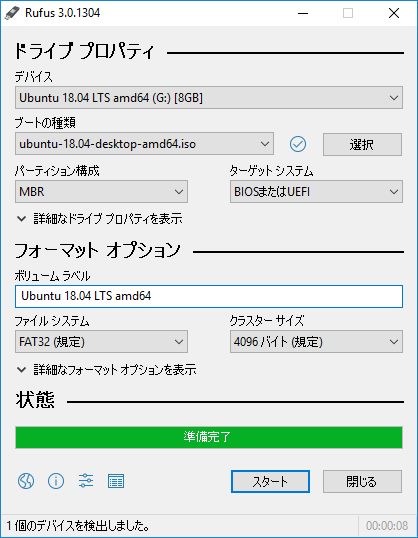
\includegraphics[width=65truemm, clip]{images/rufus_jp.png}
  \label{fig:rufus}
  \caption{Dialog of Rufus}
\end{figure}

\noindent
「デバイス」の欄にはライブUSBにするUSBメモリを選択します.
「ブートの種類」の欄には先ほどダウンロードしたUbuntu 18.04LTSのISOイメージファイルを指定します.

「スタート」ボタンをクリックすれば書き込みが開始されます.
イメージを書き込んだUSBメモリの中身は全て消去されます.
重要なファイルが入っている場合は事前にバックアップを取っておきましょう.

無事にライブUSBが作成できたら,いよいよUbuntuのインストール作業に入ります.

\subsection{Ubuntuのインストール}

作成したライブUSBをNUCに接続し,ディスプレイやキーボード等を繋いでNUCを起動します.
「Install Ubuntu」を選択して,Ubuntuのインストールを開始します.
Ubuntuのインストールはウィザードの指示に従って作業を行えば大丈夫です.

\end{document}